% !TeX spellcheck = en_US
\documentclass[11pt]{article}

\usepackage[hmargin=3.1cm,vmargin=2.4cm]{geometry}
\usepackage{mathtools}
\usepackage[dvipsnames]{xcolor}
\usepackage{amssymb,dsfont,stmaryrd}
\usepackage{algorithm2e}
\usepackage{hyperref,cleveref}
\usepackage{graphicx}
\usepackage{booktabs}
\usepackage{subcaption}
\usepackage{titlesec}


\hypersetup{
	colorlinks,
	urlcolor=NavyBlue
}

%%% Math macros %%%

\newcommand\RR{\mathbb{R}}
\newcommand\CC{\mathbb{C}}
\newcommand\ZZ{\mathbb{Z}}
\newcommand\NN{\mathbb{N}}
\newcommand\TT{\mathbb{T}}
\newcommand\PP{\mathbb{P}}
\newcommand\EE{\mathbb{E}}
\DeclarePairedDelimiter{\intinterv}{\llbracket}{\rrbracket}

\renewcommand{\epsilon}{\varepsilon}

\newcommand{\suchthat}{\mathrm{s.t.}}

\DeclareMathOperator*{\argmin}{\mathrm{argmin}}
\DeclareMathOperator*{\argmax}{\mathrm{argmax}}
\DeclareMathOperator{\diag}{\mathrm{diag}}
\DeclareMathOperator{\sgn}{\mathrm{sgn}}
\DeclareMathOperator{\trace}{\mathrm{Tr}}

\newcommand{\calM}{\mathcal{M}}
\newcommand{\calP}{\mathcal{M}}
\newcommand{\calN}{\mathcal{N}}
\newcommand{\calX}{\mathcal{X}}
\newcommand{\calL}{\mathcal{L}}
\newcommand{\calC}{\mathcal{C}}
\newcommand{\calD}{\mathcal{D}}

\newcommand{\bmmu}{\boldsymbol{\mu}}
\newcommand{\bmpsi}{\boldsymbol{\psi}}
\newcommand{\bmphi}{\boldsymbol{\phi}}


%%% Section titling setup %%%

\titleformat*{\section}{\LARGE\bfseries\sffamily}
\titleformat*{\subsection}{\Large\bfseries\sffamily}

\titleformat{\paragraph}[runin]{\sffamily\bfseries}{}{}{}[.]


%%% Document title %%%

\title{
	MVA -- Probabilistic Graphical Models\\
	{\color{NavyBlue}\sffamily Homework 2}
}

\author{
	Wilson \textsc{Jallet}\thanks{\url{wilson.jallet@polytechnique.org}}}


\begin{document}

\maketitle

\section{K-means and the EM algorithm}

\paragraph{Question 1} We consider a mixture model of $K$ components for a dataset $(X_i)$ where $X_i\in\RR^d$. We denote $Z_i \in \{1,\ldots,K\}$ the latent hidden label. Each component occurs with probability $p_k = \PP(Z_i = k)$ and is distributed as
\[
	X_i \sim \calN(\mu_k, D_k)
\]
i.e. $p(x|k) = \frac{1}{((2\pi)^d |D_k|)^{1/2}} \exp(-\frac{1}{2} (x-\mu_k)^T D_k^{-1}(x - \mu_k))$.

The data log-likelihood under parameters $\Theta = ((p_1, \mu_1,D_1),\ldots,(p_K,\mu_K,D_K))$ is
\[
	\calL(X_1,\ldots,X_n; \Theta) =
	\sum_{i=1}^n \log\left(
		\sum_{k=1}^K p_k p(X_i | k; \mu_k, D_k)
	\right)
\]
We seek to compute the MLE
\[
	\widehat\Theta\in \argmax_\Theta \calL(X_1,\ldots,X_n;\Theta)
\]
This optimization problem is intractable when using straightforward methods.

The EM algorithm goes as follows:
\begin{itemize}
	\item \textit{\underline{Expectation}} Compute the posterior probability of the latent variables $Z_i$:
	\begin{equation}
	q^{(t)}_{k,i} = p(Z_i = k|X_i;\Theta^{(t)}) =
	\frac{
		p^{(t)}_k p(X_i|Z_i=k; \Theta^{(t)})
	}{
		\sum_{\ell=1}^K p^{(t)}_\ell p(X_i|Z_i=\ell; \Theta^{(t)})
	}
	\end{equation}
	and denote $w_k^{(t)} = \sum_{i=1}^n q_{k,i}^{(t)}$ -- we then have $\sum_{k=1}^K w_k^{(t)} = n$.
	\item \textit{\underline{Maximization}} Update the parameters $\Theta^{(t)}$ by maximizing the lower bound objective:
	\begin{equation}
	\max_{\Theta}~
	\mathcal{J}(q^{(t)}, \Theta) =
	\sum_{i=1}^n \left(
	\sum_{k=1}^K q^{(t)}_{k,i}
	\left(
		\log p_k
		- \frac{d}{2}\log(2\pi)
		- \frac{1}{2}\log{|D_k|}
		- \frac{1}{2}(X_i - \mu_k)^T D_k^{-1}(X_i-\mu_k)
	\right)
	\right)
	\end{equation}
	subject to $\sum_{k=1}^K p_k = 1$ (associated to a multiplier $\nu$). The KKT conditions give the null gradient condition:
	\begin{subequations}
	\begin{align}
		& \frac{1}{p_k} w_k^{(t)} - \nu = 0  \\
		& -\sum_{i=1}^n q_{k,i}^{(t)}D_k^{-1}(\mu_k - X_i) = 0  \\
		& -\frac{1}{2}
		\sum_{i=1}^n q_{k,i}^{(t)}
		(D_k^{-1} - D_k^{-2}\diag(X_i-\mu_k)^2) = 0
	\end{align}
	\end{subequations}
	Which leads to the updates:
	\begin{subequations}\label{eq:DiagEMupdate}
	\begin{align}
		p_k &= \frac{1}{n}w_k^{(t)}  \\
		\mu_k &= \frac{1}{w_k^{(t)}}
		\sum_{i=1}^n q_{k,i}^{(t)} X_i  \\
		D_k &= \frac{1}{w_k^{(t)}}
		\sum_{i=1}^n q_{k,i}^{(t)} \diag(X_i-\mu_k)^2
	\end{align}
	\end{subequations}
\end{itemize}

\paragraph{Question 2} The main advantage of this ``reduced" covariance mixture model is that it is more sparse: it uses far fewer parameters ($K(2d+1)$) than the its full counterpart, which has $K(1 + d + d(d+1)/2)$ parameters. For datasets with relatively independent features (conditionally on the latent class), this can give performance very close to the full covariance while having a smaller, simpler model (meaning better AIC or BIC scores).


\paragraph{Question 3}
\begin{figure}
	\centering
	\begin{subfigure}[t]{.95\linewidth}
		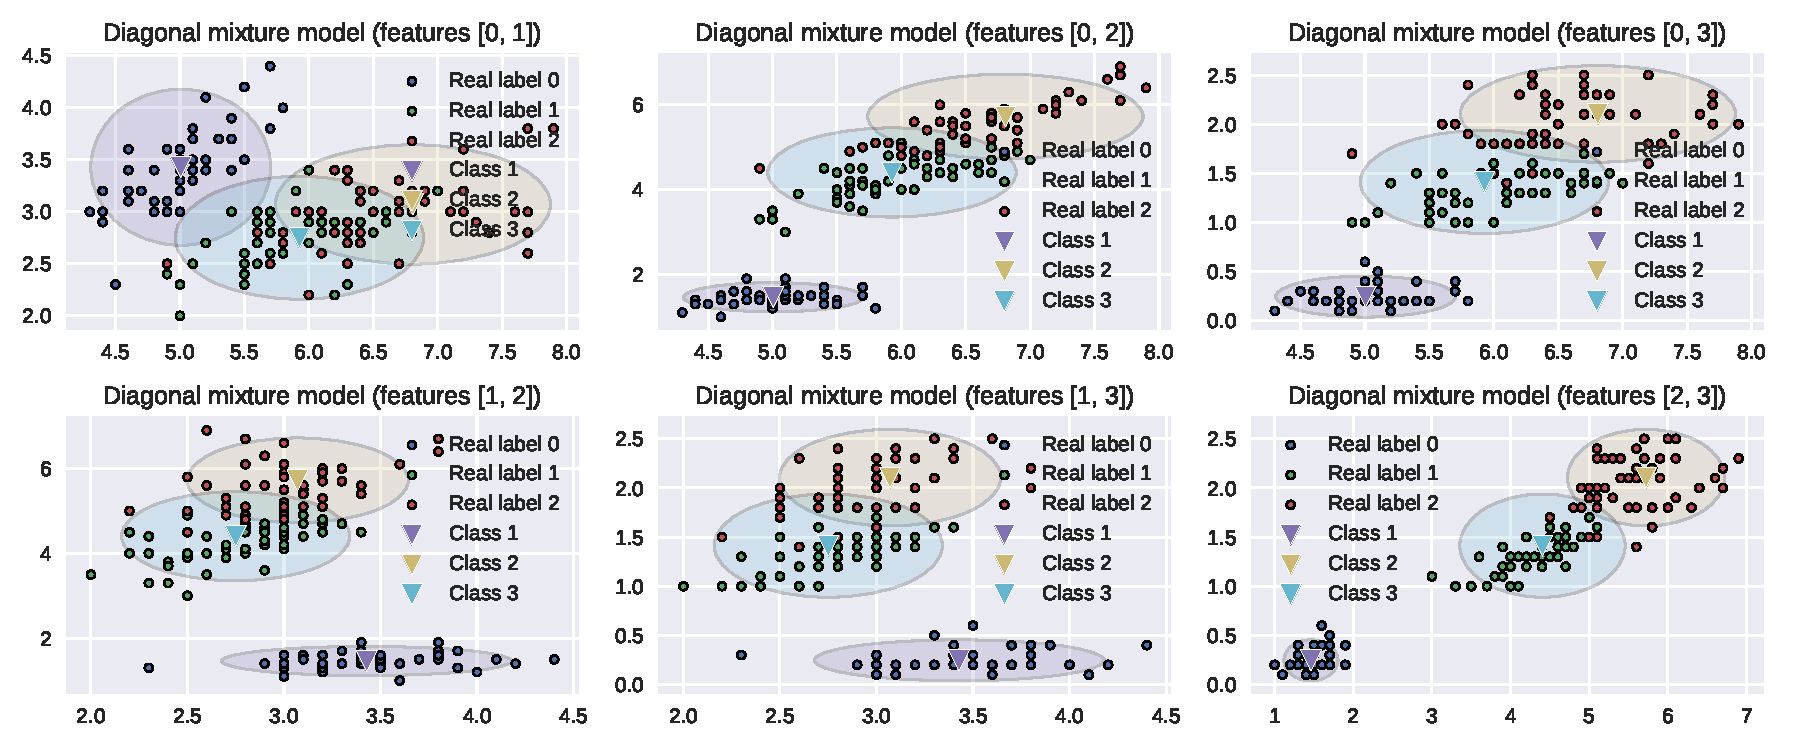
\includegraphics[width=\linewidth]{images/diag_em_K3.pdf}
		\caption{Diagonal Gaussian mixture model on the Iris dataset (our implementation). $K=3$ classes.}
	\end{subfigure}
	\begin{subfigure}[t]{.95\linewidth}
		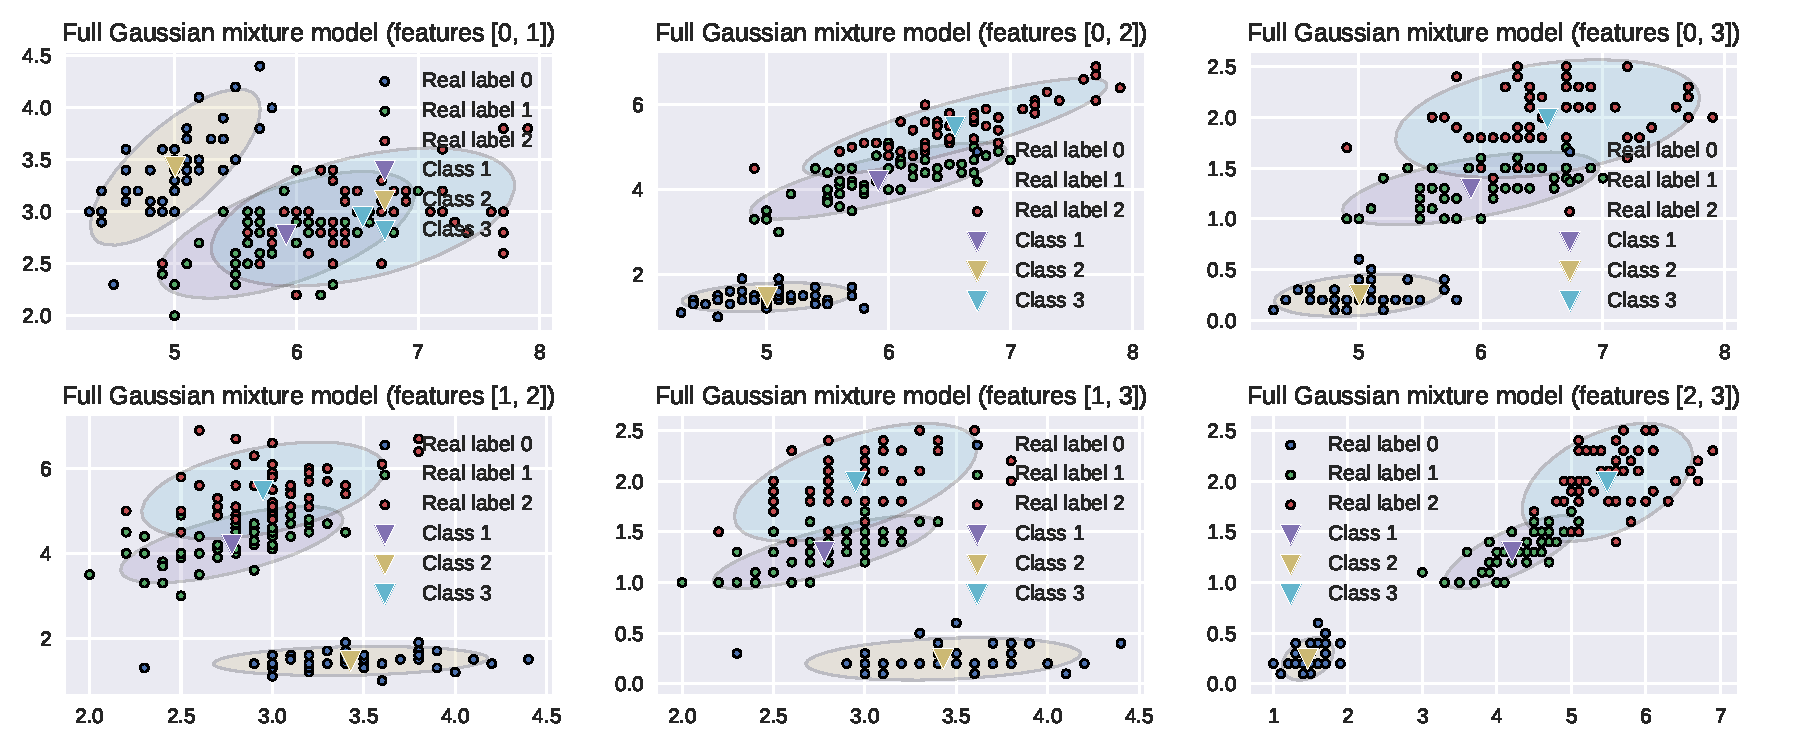
\includegraphics[width=\linewidth]{images/full_em_K3.pdf}
		\caption{Full Gaussian mixture on the Iris dataset using \texttt{scikit-learn}. $K=3$ classes.}
	\end{subfigure}
	\begin{subfigure}[t]{.95\linewidth}
		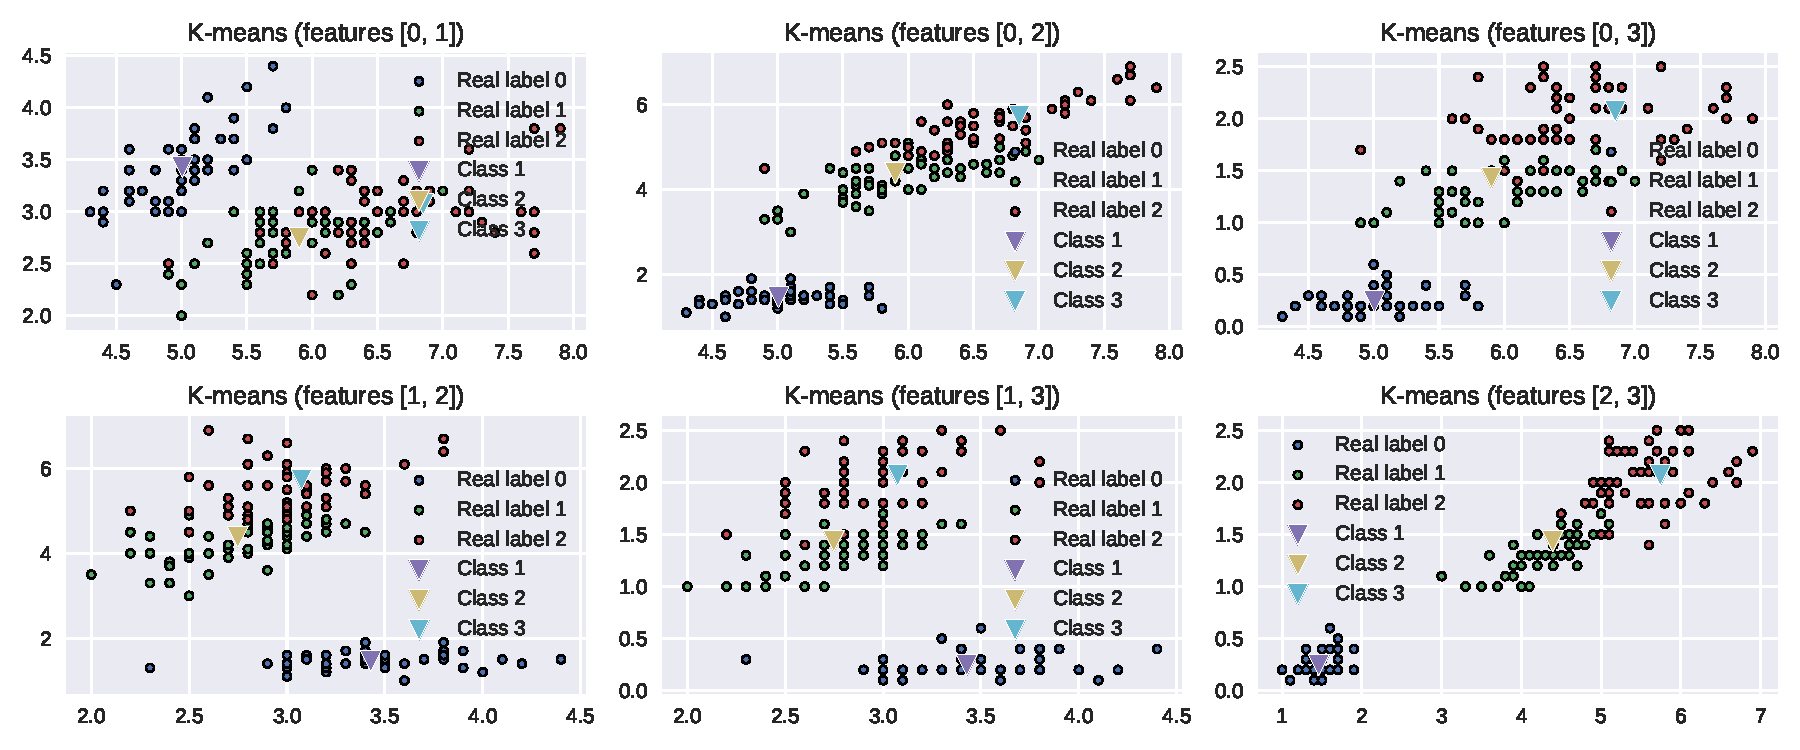
\includegraphics[width=\linewidth]{images/kmeans_K3.pdf}
		\caption{Centroids of the K-means model.}
	\end{subfigure}
	\caption{Comparison of the diagonal and full covariance mixture models and K-means for $K=3$ classes.}\label{fig:EMdiagfullComparisonK3}
\end{figure}

\begin{figure}
	\centering
	\begin{subfigure}[t]{.95\linewidth}
		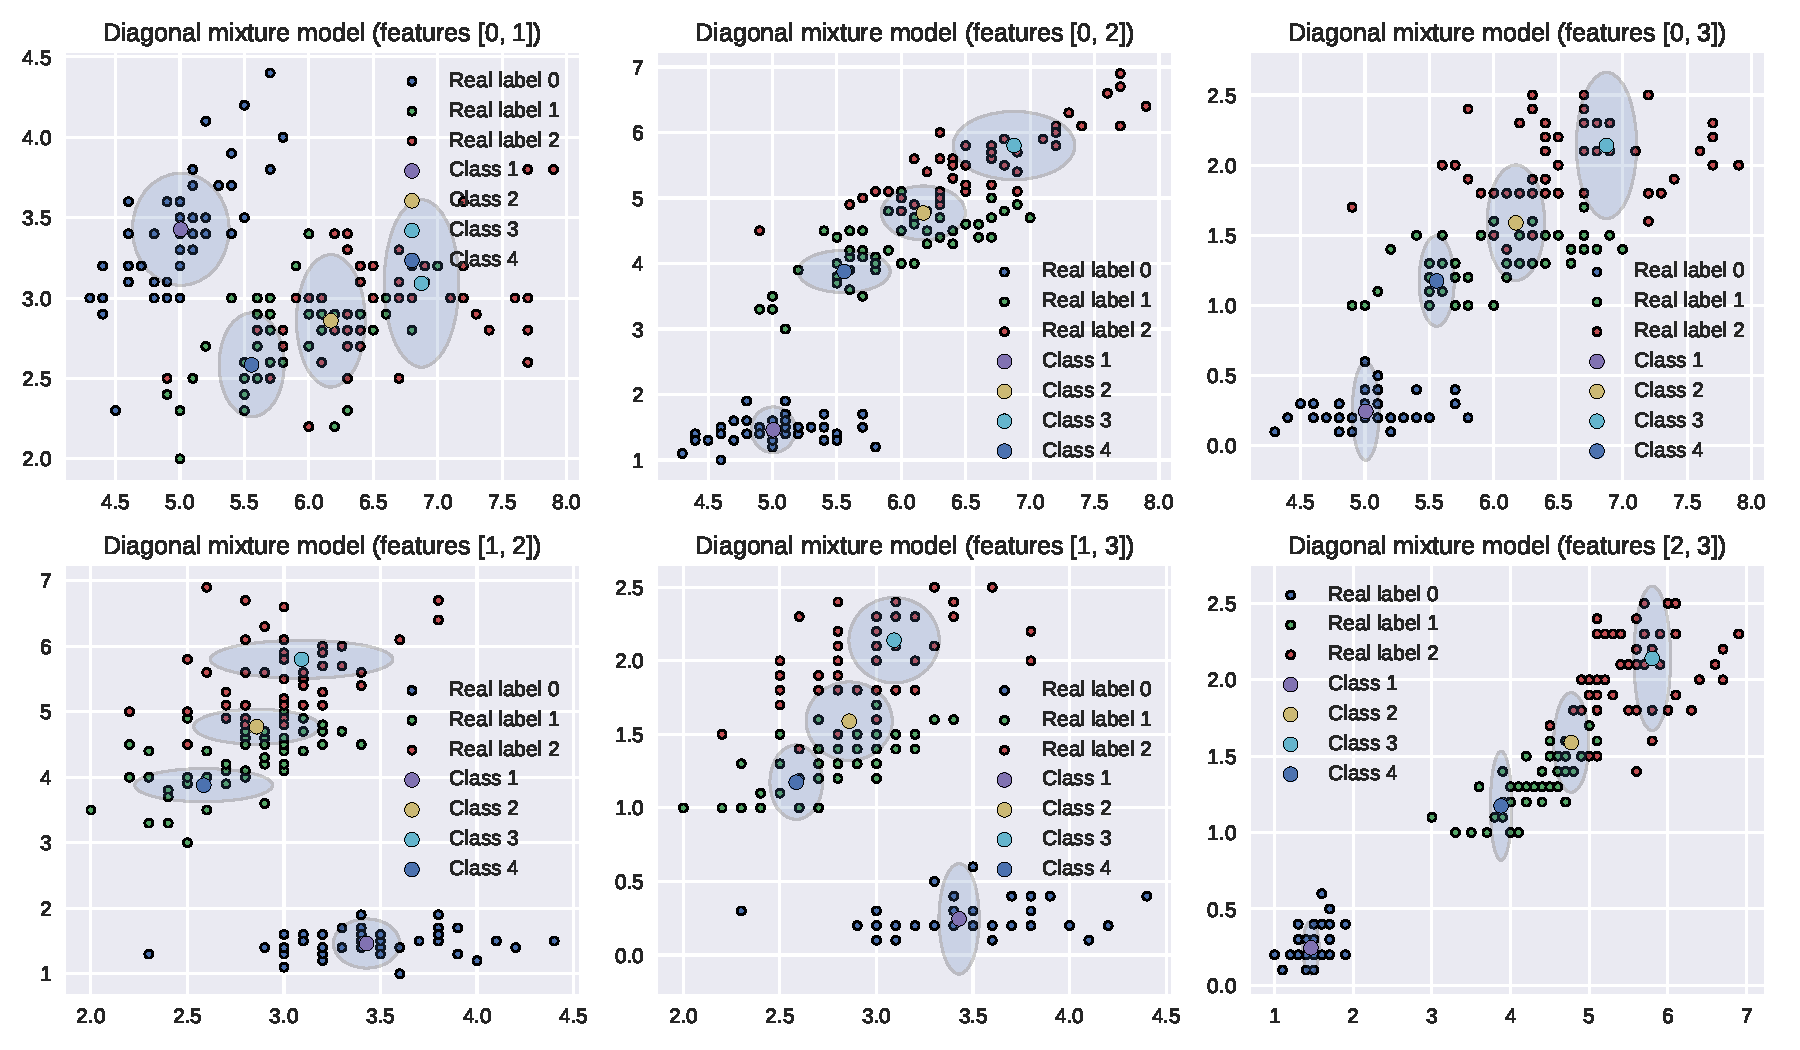
\includegraphics[width=\linewidth]{images/diag_em_K4.pdf}
		\caption{Diagonal Gaussian mixture model on the Iris dataset (our implementation).}
	\end{subfigure}
	\begin{subfigure}[t]{.95\linewidth}
		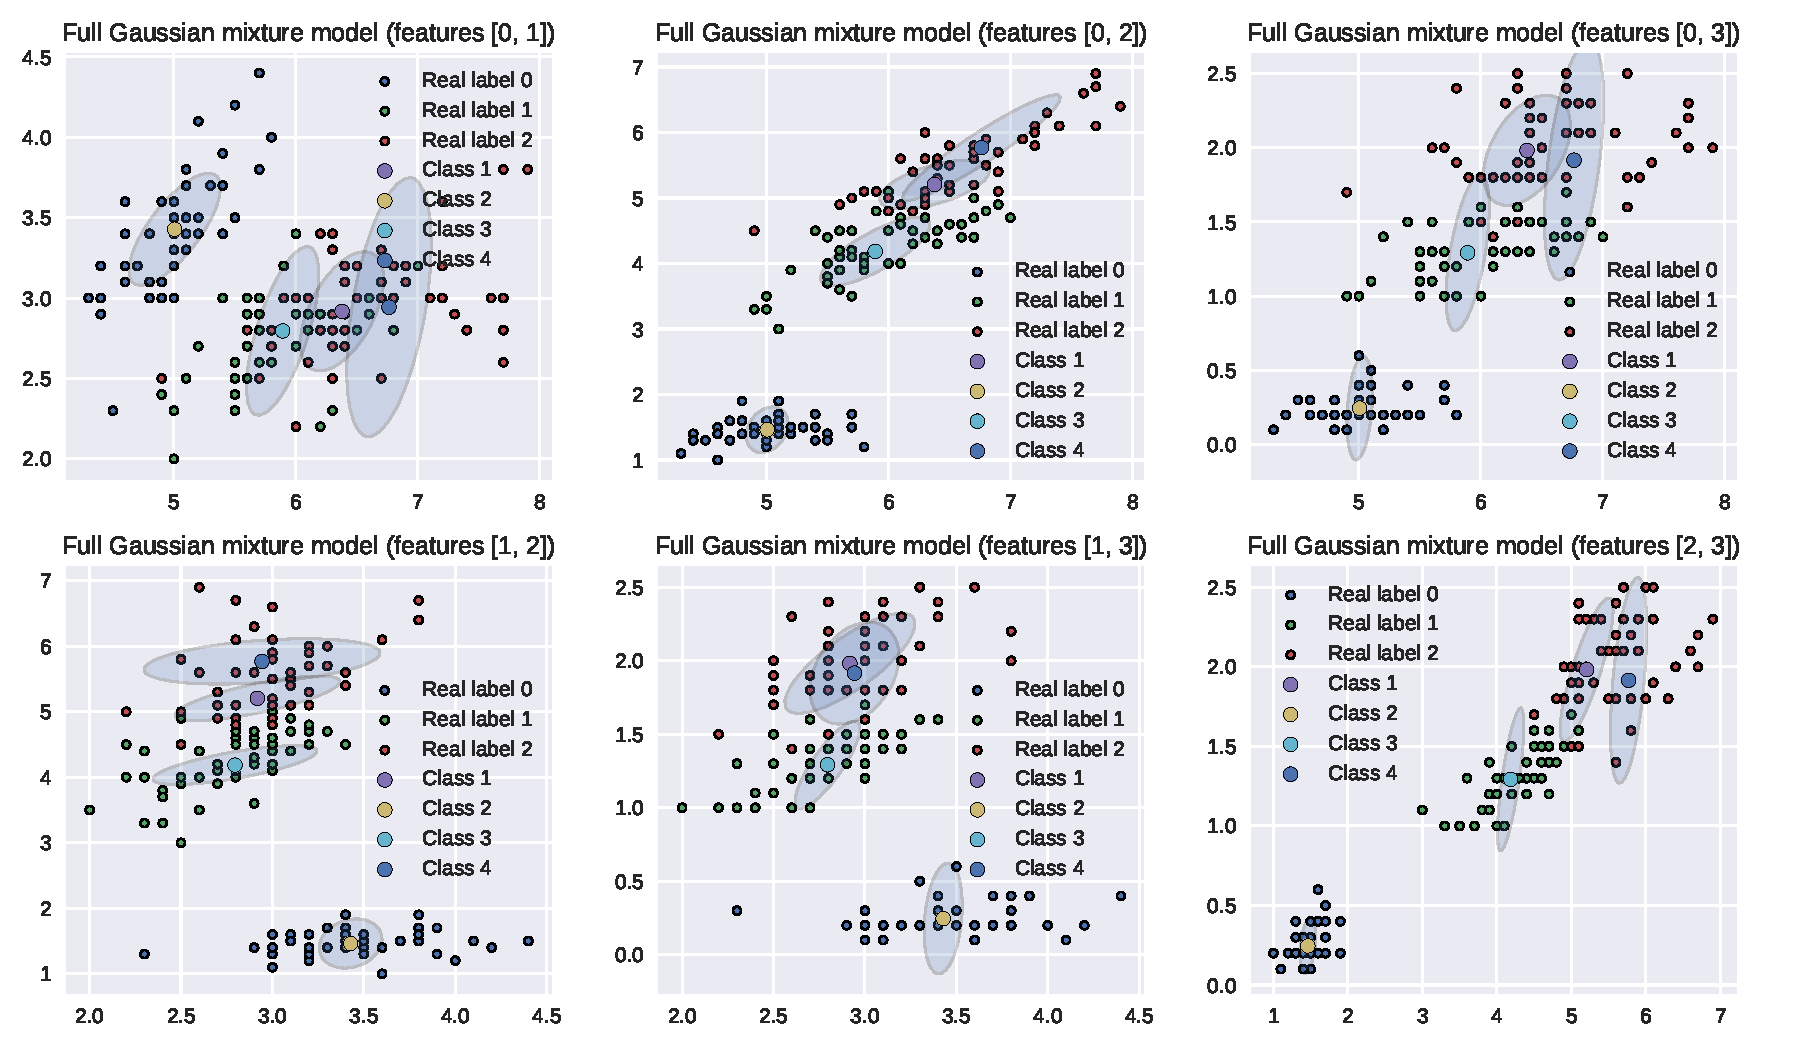
\includegraphics[width=\linewidth]{images/full_em_K4.pdf}
		\caption{Full Gaussian mixture on the Iris dataset using \texttt{scikit-learn}.}
	\end{subfigure}
	\begin{subfigure}[t]{.95\linewidth}
		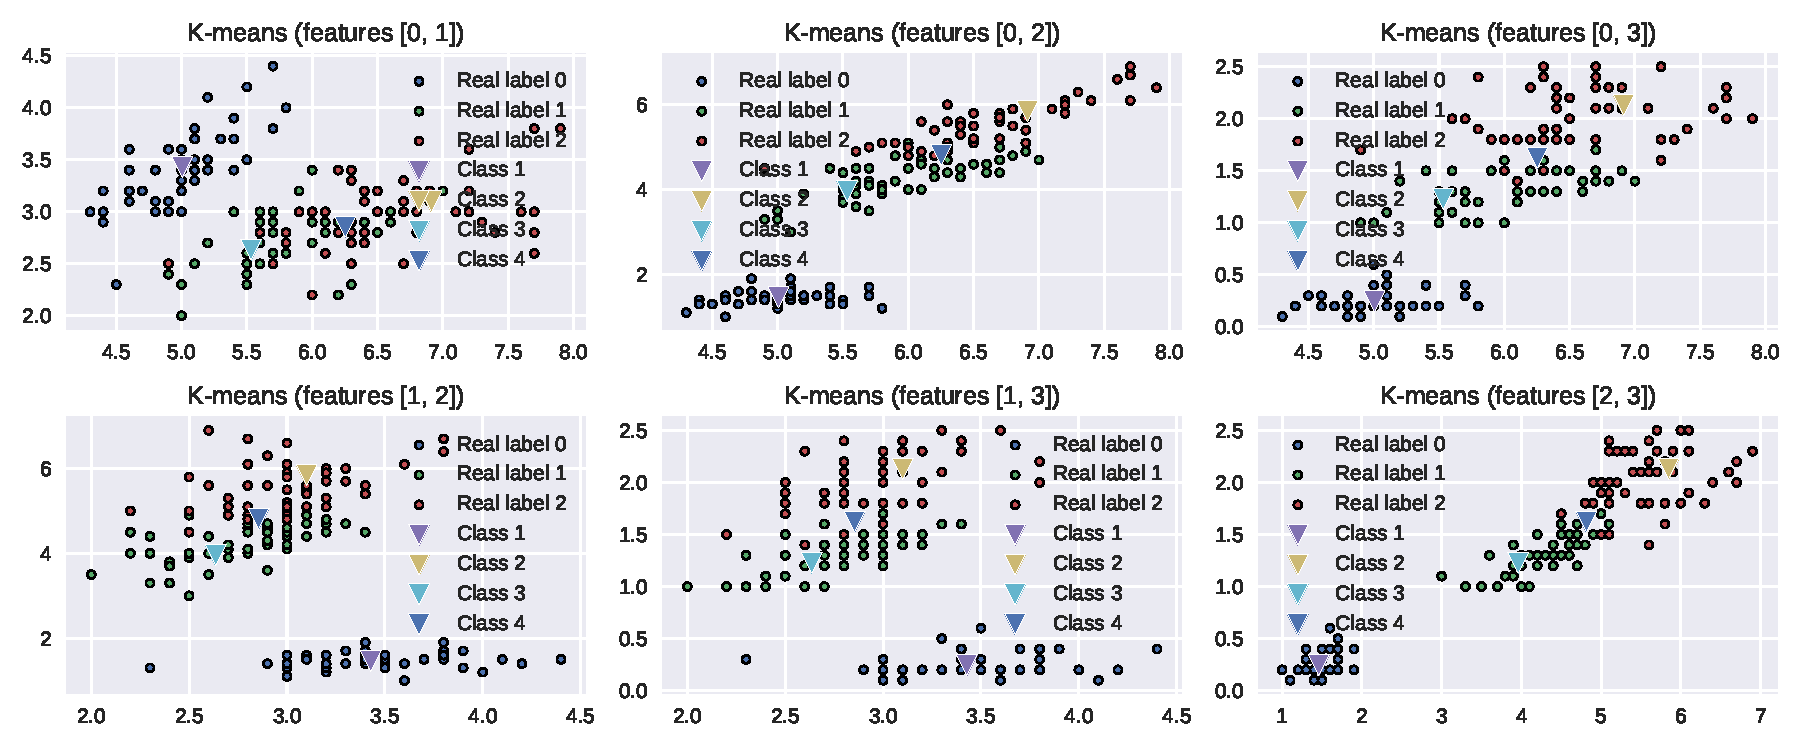
\includegraphics[width=\linewidth]{images/kmeans_K4.pdf}
		\caption{K-means.}
	\end{subfigure}
	\caption{Comparison of the models for $K=4$ classes.}\label{fig:EMdiagfullComparisonK4}
\end{figure}

\begin{figure}
	\centering
	\begin{subfigure}[t]{.95\linewidth}
		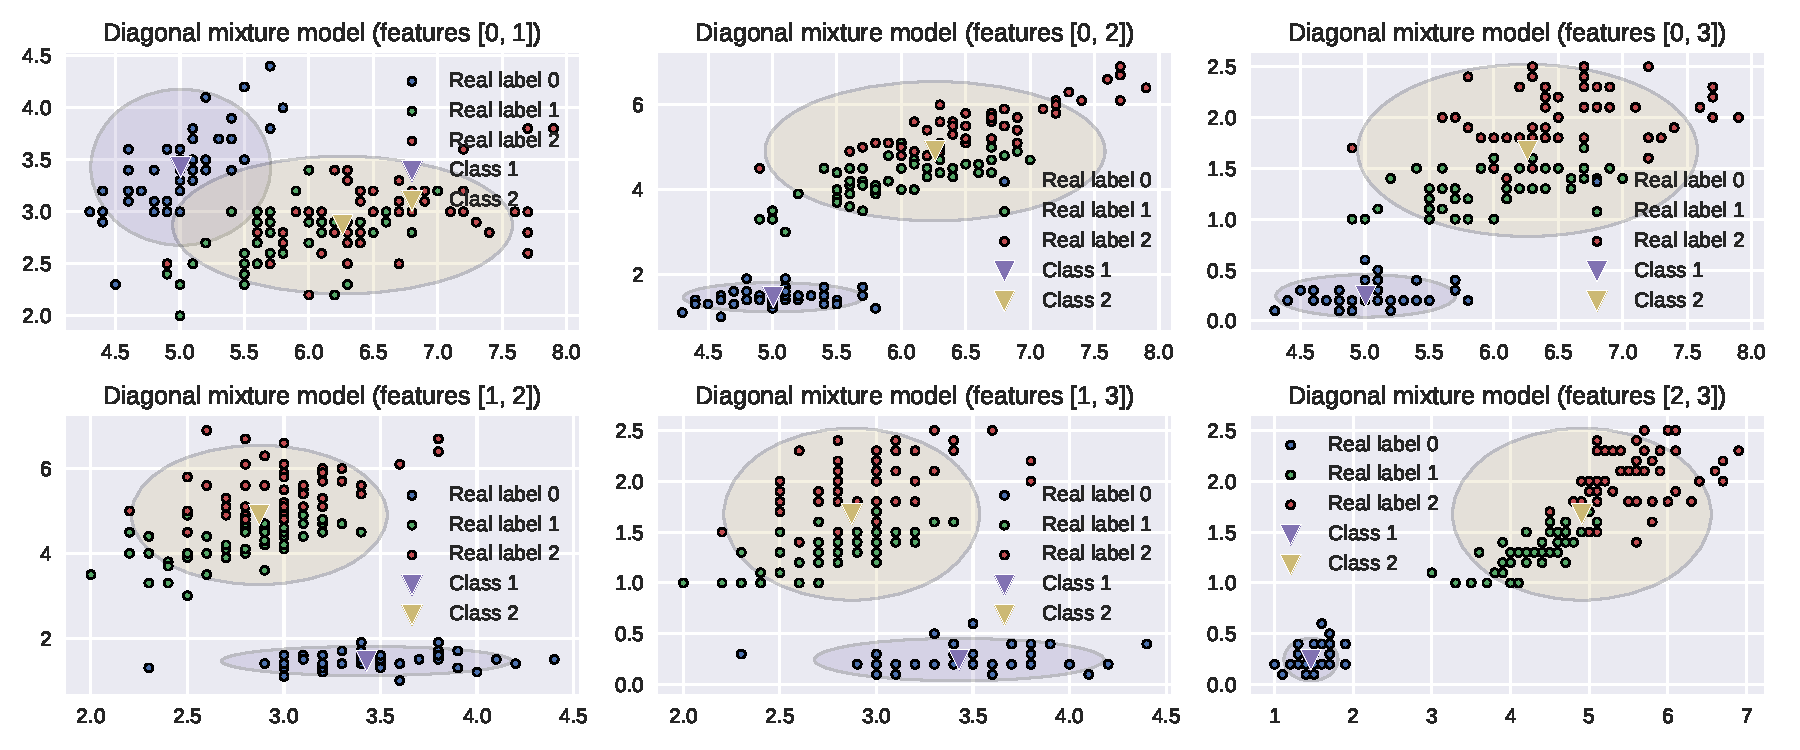
\includegraphics[width=\linewidth]{images/diag_em_K2.pdf}
		\caption{Diagonal Gaussian mixture model on the Iris dataset (our implementation).}
	\end{subfigure}
	\begin{subfigure}[t]{.95\linewidth}
		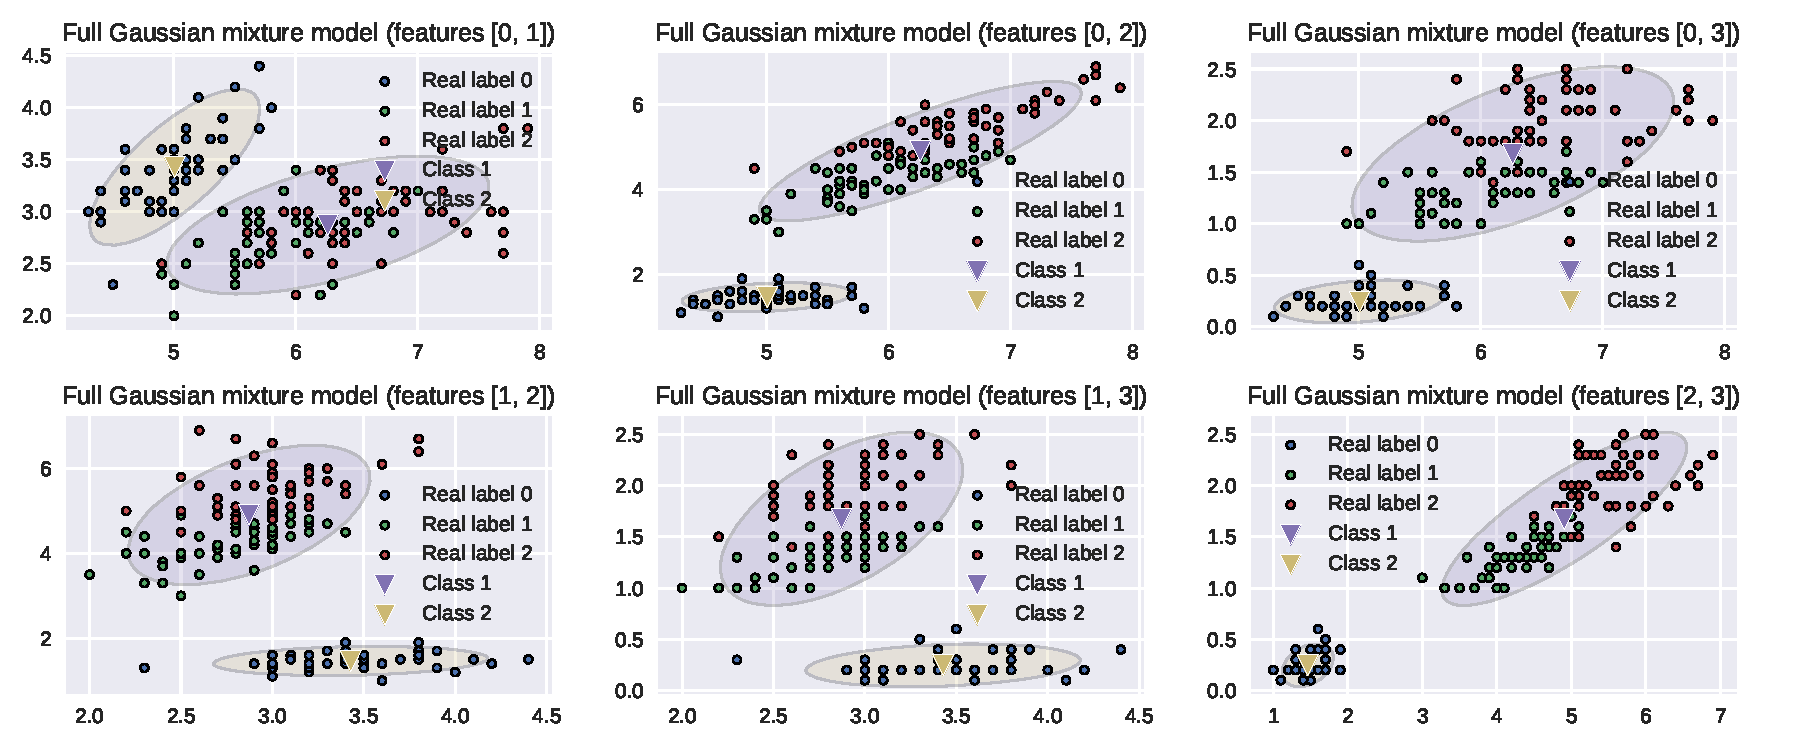
\includegraphics[width=\linewidth]{images/full_em_K2.pdf}
		\caption{Full Gaussian mixture on the Iris dataset using \texttt{scikit-learn}.}
	\end{subfigure}
	\begin{subfigure}[t]{.95\linewidth}
		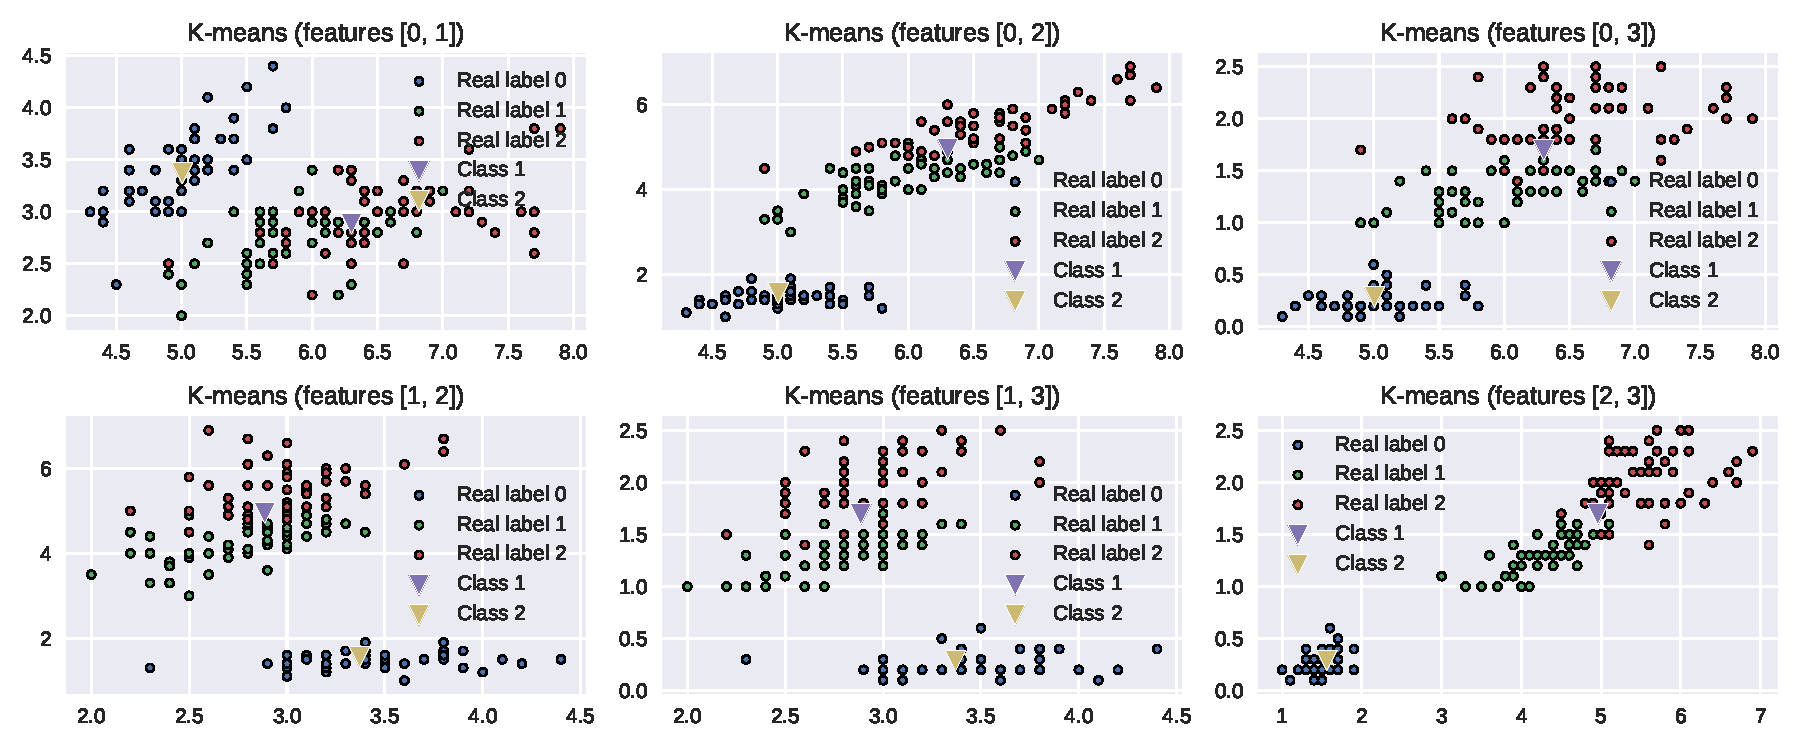
\includegraphics[width=\linewidth]{images/kmeans_K2.pdf}
		\caption{Full Gaussian mixture on the Iris dataset using \texttt{scikit-learn}.}
	\end{subfigure}
	\caption{Comparison of the models for $K=2$ classes.}\label{fig:EMdiagfullComparisonK2}
\end{figure}

\Cref{fig:EMdiagfullComparisonK3} compares the obtained latent class centroids and confidence ellipsoids (where applicable) for the diagonal and full covariance mixture models and K-means, on the Iris dataset, for a small number of classes $K=3$ (the actual number of classes in the data). \Cref{fig:EMdiagfullComparisonK2,fig:EMdiagfullComparisonK4} represent the same for $K =2, 4$ classes.


\paragraph{Question 4} I created synthetic data made up of an ellipsis and annulus: \Cref{fig:SynthDataComparison} shows how the mixture models and K-means compare.
\begin{figure}
	\centering
	\begin{subfigure}[t]{.5\linewidth}
	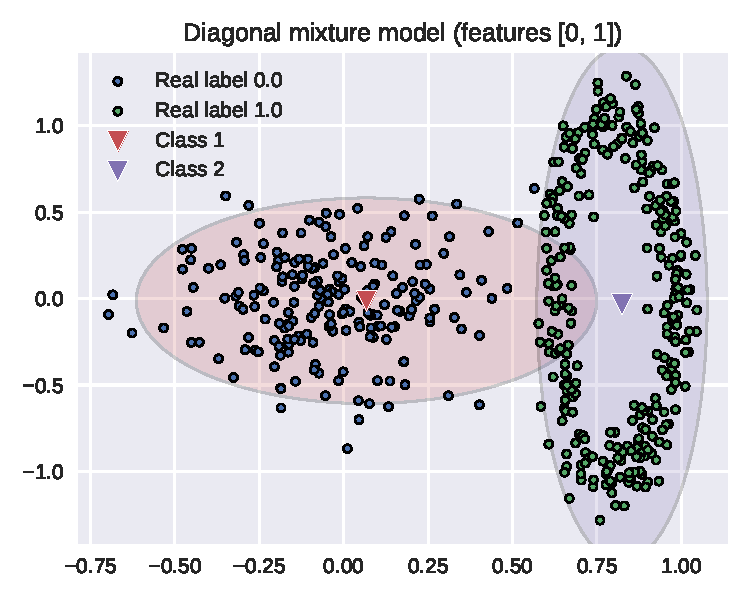
\includegraphics[width=\linewidth]{custom_data/diag_em_K2.pdf}
	\caption{Diagonal Gaussian mixture model.}
	\end{subfigure}~
	\begin{subfigure}[t]{.5\linewidth}
	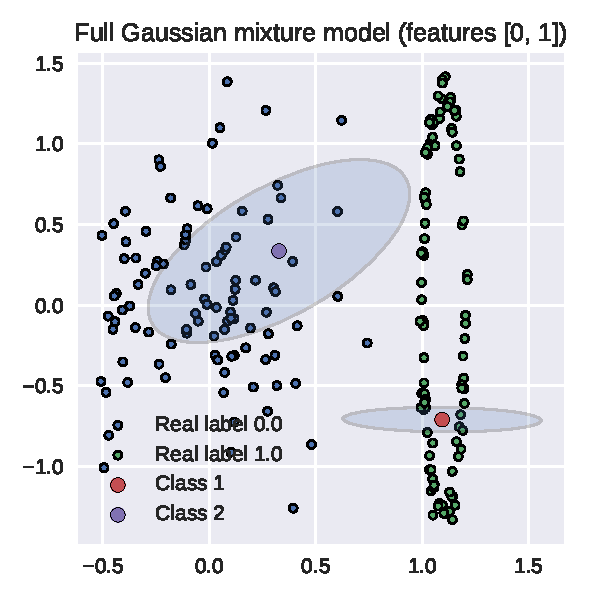
\includegraphics[width=\linewidth]{custom_data/full_em_K2.pdf}
	\caption{Full Gaussian mixture model.}
	\end{subfigure}
	\begin{subfigure}[t]{.6\linewidth}
	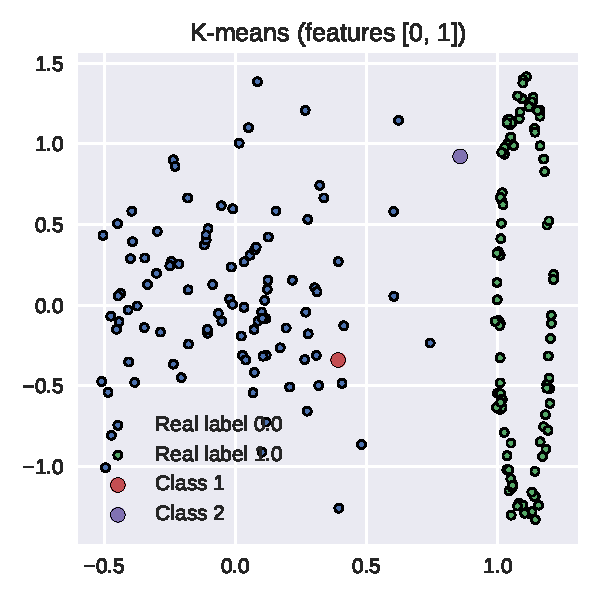
\includegraphics[width=\linewidth]{custom_data/kmeans_K2.pdf}
	\caption{Result of the K-means model: notice how the class centroids are offset from the actuel center of the class.}
	\end{subfigure}
	\caption{Comparison of the models on synthetic data where K-means performs worse than mixtures.}
	\label{fig:SynthDataComparison}
\end{figure}



\clearpage


\section{Graphs, algorithms and Ising}

\paragraph{Question 1} We recall that for an undirected chain graph $G$ probability distributions factor as
\begin{equation}
	p(x) = \frac{1}{Z}
	\prod_{i=1}^n \psi_i(x_i) 
	\prod_{i=1}^{n-1} \psi_{i,i+1}(x_i, x_{i+1})
\end{equation}

\newcommand{\LogSumExp}{\mathrm{LogSumExp}}

\textbf{The algorithm.} The marginal distribution of $X_i$ can be rewritten as
\[
	p(x_i) = \frac{1}{Z}\mu_{i-1, i}(x_i) \psi_i(x_i) \mu_{i+1, i}(x_i)
\]
where $\mu_{i-1, i}, \mu_{i+1, i}$ are (forward, backward) messages from $i-1$ to $i$ and $i+1$ to $i$. They are propagated as:
\begin{subequations}
\begin{align}
	\mu_{i, i+1}(x_{i+1}) &= \sum_{x_i}
	\psi_i(x_i)\psi_{i,i+1}(x_i, x_{i+1})
	\mu_{i-1, i}(x_i)  \\
	\mu_{i, i-1}(x_{i-1}) &= \sum_{x_i} \psi_{i}(x_i) \psi_{i-1,i}(x_{i-1}, x_i) \mu_{i+1, i}(x_i)
\end{align}
\end{subequations}


\textbf{Practical implementation.} If the state space $\calX$ of the variables $X_1,\ldots,X_n$ (for instance for binary variables) is discrete we can represent the input functions $\psi_i$ and $\psi_{i,i+1}$ as arrays. If not (continuous variables for instance), we can discretize a grid over $\calX$ and precompute an array of values for the factors.
Denoting the arrays in bold letters, we forward-propagate by
\[
	\bmmu_{i, i+1} =
	(\bmmu_{i-1, i} \odot \bmpsi_i)\bmpsi_{i,i+1}
\]
and back-propagate by
\[
	\bmmu_{i,i-1} = (\bmmu_{i,i+1} \odot \bmpsi_i) \bmpsi_{i-1,i}^T
\]
which allows to compute the marginal distributions using vectorized operations.

\Cref{fig:IndependentNodeUGM} shows an implementation for independent edges. The expected marginals are $X_1 \sim \calM(1;1/4,1/2,1/4)$, $X_2\sim \calN(0,2)$ and $X_3 \sim \mathcal{B}(1/2)$.

\begin{figure}
	\centering
	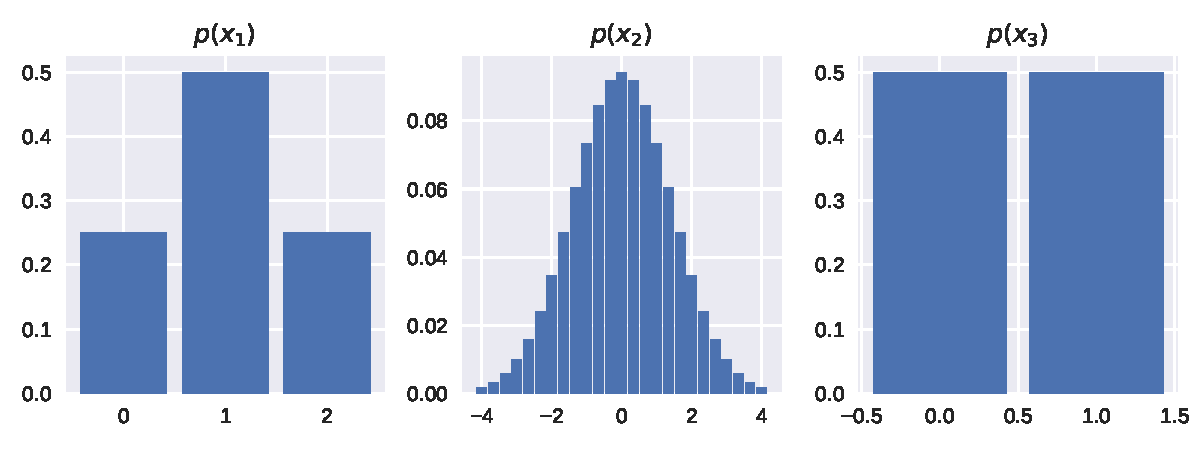
\includegraphics[width=.9\linewidth]{images/graphs/independent_undirected_chain.pdf}
	\caption{Sanity test: undirected graph with $n=3$ nodes, and a probability distribution $p$ with factors $\psi_1 = (1, 2, 1)$, $\psi_2(x_2) = \exp(-x_2^2/4)$, $\psi_3 = (1,1)$ and $\psi_{i,i+1} = 1$ (i.e. independence).}\label{fig:IndependentNodeUGM}
\end{figure}



\paragraph{Question 2} The vertex set $V$ of the graph $G = (V,E)$ induced by the grid has vertices of the form $v = (j,k)$ where $1\leq j \leq w$ and $1 \leq k \leq h$. An easy junction tree to extract from $G$ is given by collapsing the rows into supernodes: the resulting tree $T$ has vertex set $V_T = \{c_k\}$ where $c_k = \{(j,k)\}_j$ and looking at the resulting edges shows $T$ is actually an undirected chain $c_1-c_2 -\cdots-c_h$. Computationally, since there are $w=10$ columns and $h=100$ rows, this leads to a reasonably-sized state space ($2^{10}$ different states) for each supernode.

The probability factorizes using the clusters as
\begin{align*}
	p(x) &= \frac{1}{Z}\prod_k
	\phi_k(x_{c_k})
	\prod_k
	\phi_{k,k+1}(x_{c_k},x_{c_{k+1}})
\end{align*}
where 
\begin{align*}
	\phi_k(x_{c_k}) &= \prod_{j=1}^w e^{\alpha x_{(j,k)}}
	\prod_{j=1}^{w-1} e^{
		\beta \mathds{1}(
			x_{(j,k)}=x_{(j+1,k)}
		)
	}  \\
	\phi_{k,k+1}(x_{c_k}, x_{c_{k+1}}) &=
	\prod_{j=1}^w e^{
		\beta \mathds{1}(
			x_{(j,k)}=x_{(j,k+1)}
		)
	}
\end{align*}
The vector $\bmphi$ is of size $2^{10}$.

\end{document}
